\documentclass[a4paper,oneside]{book}

\usepackage{lipsum}
\usepackage[hidelinks]{hyperref}
\usepackage[a4paper, total={7.27in, 10.69in}]{geometry}
\usepackage{titletoc}
\usepackage{graphicx}
\titlecontents*{chapter}
  [0pt]% <left>
  {}
  {\chaptername\ \thecontentslabel\quad}
  {}
  {\bfseries\hfill\contentspage}    

\usepackage{bookmark}
\usepackage{etoolbox}

\makeatletter
\newcommand*{\AddChapterPrefixInBookmarks}{%
  \if@mainmatter
    \ifnum\bookmarkget{level}=0 %
      \preto\bookmark@text{\@chapapp\space}%
    \fi
  \fi
}
\makeatother

\bookmarksetup{
  numbered,
  addtohook=\AddChapterPrefixInBookmarks,
}

% Workaround for numbered sections in unnumbered
% chapter "Introduction" to avoid chapter number
% zero.
\renewcommand*{\thesection}{%
  \ifcase\value{chapter}%
  \else
    \thechapter.%
  \fi
  \arabic{section}%
}

\title{My document}
\pagestyle{headings}

\begin{document}
\frontmatter

\begin{titlepage}
    \begin{center}
        \vspace*{1cm}
            
        \Huge
        \textbf{Statistics Question Bank}
            
        \vspace{0.5cm}
        \LARGE
        First Paper
            
        \vspace{1.5cm}
            
        \textbf{Abdullah Al Mahmud}
            
        \vfill
            
            
        \vspace{0.8cm}
            
 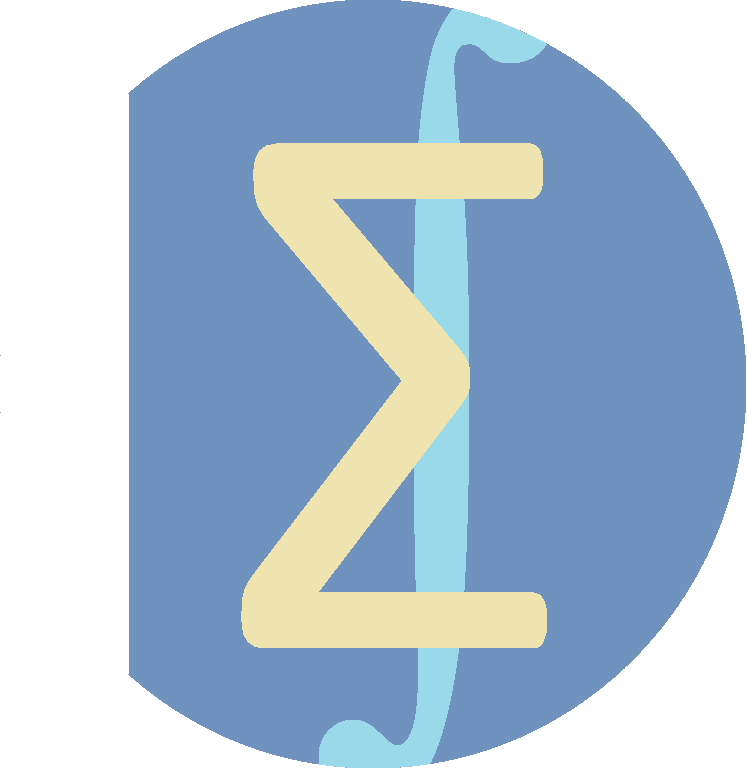
\includegraphics[width=1cm]{logo}
 
        \Large
        www.statmania.info\\
            
    \end{center}
\end{titlepage}

\tableofcontents


\mainmatter

\chapter{Statistics, Variable and Concepts of Different Symbols} 

\section{Creative Questions}

\begin{enumerate}

\item
	  \textbf{Goals scored by a footballer in 25 matches are summarized as shown below.} 
	  
	  \begin{table}[h]
	  \centering
\begin{tabular}{|c|ccccc|}
Goals & 0 & 1 & 2 & 3 & 4 \\ \hline
Times & 8 & 9 & 5 & 2 & 1
\end{tabular}
\end{table}
  
  \begin{enumerate}
    \item
	Is no. goals a discrete or continuous variable? \hfill 1
    \item
	Verify theoretically: $\displaystyle \sum_{i=2}^{2} X_iY_i = \sum_{i=1}^{2} X_i \times \sum_{i=1}^{2} Y_i$ \hfill 2
    \item  
	Find the total number of goals using a suitable notation. \hfill 3
    \item
	If he scores two (2) goals in the next match, will the scoring rate increase? \hfill 4
  \end{enumerate}

 \item
	  \textbf{Height (in inches) of 10 cadets in a class are: 50, 60, 55, 65, 66, 70, 54, 64, 62, 72} 
	 
  \begin{enumerate}
    \item
	What is population in statistics? \hfill 1
    \item
	Is height discrete or continuous? \hfill 2
    \item  
	Find $\displaystyle \sum_{i=1}^{10} x_i^2$ \hfill 3
    \item
	Find the square of mean and mean of square. Are they equal? \hfill 4
  \end{enumerate}
  
   \item
	  \textbf{Marks of 10 students in Statistics in a class were found to be the following:} 
	 
	 \begin{center} 
	  99, 88, 98, 85, 97, 71, 87, 79, 70, 84
	  
	  \end{center}
	  
	  Later it was discovered that all marks should be 5 less than the recorded marks. 
  
  \begin{enumerate}
    \item
	What is change of origin? \hfill 1
    \item
	Does summation of a variable depend an change of origin?  \hfill 2
    \item  
	Considering the data in stem as X, find $\displaystyle \sum_{i=1}^{10} X_i$ and $\displaystyle \sum_{i=1}^{10} (X_i+3)$ \hfill 3
    \item
	Find the arithmetic mean of the corrected values, employing the concept of shift of origin. \hfill 4
  \end{enumerate}

  \item
  \textbf{Income and expenditure (both in thousands) of some individuals in four successive months are collected:}
 
\begin{table}[h]
 \begin{center}
\begin{tabular}{l|l|l|l|l}

Income (x)  & 20 & 30 & 25 & 10 \\ \hline
Expenditure (y) & 15  & 27  & 18 & 5 \\ 
\end{tabular}
\end{center}
\end{table}


  \begin{enumerate}
    \item
	What is a discrete variable? \hfill 1
    \item
    	Can fractional numbers be discrete? Explain briefly.  \hfill 2
    \item
    	Are, in the stem, $\displaystyle \sum_{i=1}^{n} \sum_{i=1}^{n} x_iy_j = \sum_{i=1}^{n} x_iy_i?$ Vindicate \hfill 3
     \item
     	Using data, prove  that sum of square is unequal to square of sum of numbers. \hfill 4
  \end{enumerate}
  
   \item
  \textbf{Call duration of 6 calls in a customer care center are}
  
  \begin{center}
  2, 2.5, 1.5, 5, 6, 3
  \end{center}
 
  \begin{enumerate}
    \item
	What is a sample? \hfill 1
    \item
    	Are all quantitative variables continuous?  \hfill 2
    \item
    	Determine $\displaystyle \sum_{i=1}^7 (x_i-3)^3$ \hfill 3
     \item
     	Find the values of  $\displaystyle \sum_{i=1}^7 (x_i-5)^2$ and $\displaystyle \sum_{i=1}^7 x_i^2+5.$  \hfill 4 \\
     	Explain mathematically why they are unequal.
  \end{enumerate}
  
   \item
	  \textbf{Goals scored by Karim Benzema in five seasons are recorded to be the following:} 
	  
	  \begin{table}[h]
	  \centering
\begin{tabular}{c|c|c}
Season & La Liga (x) & Uefa Champions League (y) \\ \hline
2017-18 & 5 & 5 \\ 
2018-19 & 21 & 4 \\
2019-20 & 21 & 5 \\
2020-21 & 23 & 6 \\ 
2021-22 & 27 & 15 \\ \hline
\end{tabular}
\end{table}
  
  \begin{enumerate}
    \item
	What is a quantitative variable? \hfill 1
    \item
	What is the notation to denote his total number of goals? \hfill 2
    \item  
	Compute $\displaystyle \sum_{i=1}^5 (y_i - 3)^2$ \hfill 
    \item
	Find total number of goals using two different notations and examine whether they match. \hfill 4
  \end{enumerate}

  
 \item
	  \textbf{Below are some information} 
  
  $x_1=3, x_2=4, x_3=1, x_4=0 \\
	  y_1=1, y_2=5, y_3=0, y_4=2$
  
  \begin{enumerate}
    \item
	What is a qualitative variable? \hfill 1
    \item
	Find $\displaystyle \sum_{i=1}^{4}x_i^2$ \hfill 2
    \item  
	Prove that $\displaystyle \sum_{i=1}^{4} (x_i+y_i) = \sum_{i=1}^{4}x_i + \sum_{i=1}^{4}y_i $ \hfill 3
    \item
	Find the value of $\displaystyle \sum_{i=1}^{4} x_iy_i-\sum_{i=1}^{4} x_i+4$ \hfill 4

  \end{enumerate}
  
   \item
	  \textbf{An analyst obtains some data:}
	  \begin{center}
	  $x_1=15, x_2=-12, x_3=17, x_4=11, x_5=23$
  \end{center}
  \begin{enumerate}
    \item
	What is sample? \hfill 1
    \item
	Briefly explain shift or origin and scale. \hfill 2
    \item  
	Compute the value of $\displaystyle \sum_{i=1}^5 (x_i-10)^2$ \hfill 3
    \item
	Find the value of $\displaystyle \sum_{i=1}^5 (5x_i^2-4x_i-3)$ and examine its dependency on origin and scale. \hfill 4
  \end{enumerate}

  
  \end{enumerate}

\section{Short Questions}
\begin{enumerate}
    \item
	$x_1=2, x_2=-3, x_3=7, x_4=12.$ 
	
	Find the values of the following: \hfill $4 \times 1.5 = 6$
	
	i) $\displaystyle \sum_{i=1}^3 x_i$ 
	ii) $\displaystyle \sum_{i=1}^4 x_i^2$
	iii) $\displaystyle \sum_{i=1}^4 (x_i+3)$
	iv) $\displaystyle \sum_{i=1}^4 (x_i-4)^2$
	
	
	\item \textbf{Write down the scales of measurement of the following variables.} \hfill $8 \times 0.5 = 4$

	Gender, Religion, Temperature, Income group (Lower class, Low, Middle, High)
	
Income, Distance of stars, Radius of screws, Room no.

\item \textbf{Distinguish between the qualitative and quantitative variable.} \hfill $6 \times 0.5 = 3$

Diameter of trees, Color, Weight, Gender, Jersey Number, Family Size

\item \textbf{Distinguish between the discrete and continuous variable.} \hfill $8 \times 0.5 = 4$

Number of vote cast for a particular candidate, Time required to run 100 m, Years of schooling, Number of goals in a soccer match, Body temperature, Gravity of stars, Absolute humidity, Atomic Number

\end{enumerate}

\chapter{Collection, Presentation, and Organization of Data} 

\section{Creative Questions}

    \begin{enumerate}
    
     \item
	  \textbf{Favorite colors of 30 individuals are noted down. There are five different colors. The recorded colors are given below:}
	  
	  \begin{centering}
	  Brown Red   Pink  Green Green Green Brown Pink  Brown Red   \\
    Brown Red   Green Pink  White Red   Brown Green White Brown \\
    White Brown Pink  Red   White Brown Green Red   Pink  Red  \\
    \end{centering}
    
  
  \begin{enumerate}
    \item
	What is nominal data? \hfill 1
    \item
	What are the ways to deal with categorical data? \hfill 2
    \item  
	Draw a Pie Chart from the above data and explain. \hfill 3
    \item
	Is Bar Diagram a better representation of this data? Justify. \hfill 4
  \end{enumerate}
  
     \item
	  \textbf{Hourly wages of 100 workers in an idustry were collected by a market analyst. The analyst desires to mine a pattern and useful insights from the collected data about the industry. The obtained data are demonstrated below:}
	  
	  \begin{table}[h]
	  \centering
\begin{tabular}{c|c|c|c|c|c|c|c}
Wage              & 51-55 & 56-60 & 61-65 & 66-70 & 71-75 & 76-80 & 81-85 \\ \hline
Number of workers & 7     & 11    & 18    & 36    & 15    & 8     & 5    
\end{tabular}
\end{table}

  \begin{enumerate}
    \item
	What is class interval? \hfill 1
    \item
	How does a frequency distribution help us to find pattern in data? \hfill 2
    \item  
	Draw an Ogive from the data provided and explain. \hfill 3
    \item
	Write five useful insights about the data combining information from Ogive and the table. \hfill 4
  \end{enumerate}
  
    \end{enumerate}
    
\section{Short Questions}

\chapter{Measures of Central Tendency} 
\section{Creative Questions}
\begin{enumerate}

 \item
	  \textbf{Scores by Travis Head in the last two matches of ICC Men's Cricekt World - 2023 are given. In Cricket, Strike Rate (SR) is computed by dividing Balls by Runs and then multiplying the quotient by 100.} 
	  
	  \begin{table}[h]
	  \centering
\begin{tabular}{c|c|c}
Match & Runs & Balls \\ \hline 
1 & 62 & 48 \\
2 & 137 & 120 \\ \hline 
\end{tabular}
\end{table}
  
  \begin{enumerate}
    \item
	How many averages do you know of? \hfill 1
    \item
	Give an example when arithmetic mean is appropriate instead of harmonic mean. \hfill 2
    \item  
	When is Weighted Harmonic mean is used. Show a numerical example. \hfill 3
    \item
	Determine the average Strike Rate of the batter \hfill 4
  \end{enumerate}
  
   \item
	  \textbf{Average height of the four tallest towers in Dhaka is 153.25 meters. The heights of first three towers is 171, 153 and 152 meters, respectively. A new tower has been built with height 150 meters.} 
  
  \begin{enumerate}
    \item
	Write two primary uses of central tendency. \hfill 1
    \item
	Prove mathematically: $\displaystyle \sum_{i=1}^n (x_i-\bar x) = 0$ \hfill 2
    \item  
	Compute the height of the forth tower. \hfill 3
    \item
	After the addition of the new tower, will the average increase or decrease? Explain logically and empirically (using data). \hfill 4
  \end{enumerate}

 \item
	  \textbf{For two non-zero positive numbers, $GM=4\sqrt3$ and $HM=6$, where the quantities bear usual notations} 
  
  \begin{enumerate}
    \item
	When is Harmonic mean suitable? \hfill 1
    \item
	For two numbers, what is the relationship between AM, GM, and HM? \hfill 2
    \item  
	What is the Arithmetic mean? \hfill 3
    \item
	Determine the numbers. \hfill 4
  \end{enumerate}
  
   \item
	  \textbf{12 is deducted from each value of a variable and then divided by 3. The new arithmetic mean (AM) is found to be 4.} 
  
  \begin{enumerate}
    \item
	What is change of origin? \hfill 1
    \item
	Does AM depend on origin? Prove with an example. \hfill 2
    \item  
	From the stem, find the original AM. \hfill 3
    \item
	Does the origin or the scale have greater impact on AM in this example? \hfill 4
  \end{enumerate}

   \item
	  \textbf{The arithmetic and geometric means of ages two boys Abir and Abid are 10 and 8.} 
  
  \begin{enumerate}
    \item
	What is arithmetic mean? \hfill 1
    \item
	When can we not calculate arithmetic mean? \hfill 2
    \item  
	Determine the ages of Abir and Abid. \hfill 3
    \item
	Does the data comply with the theorem $\displaystyle AM \times  = GM^2$? \hfill 4
  \end{enumerate}
  
     \item
	  \textbf{Income of 100 individuals in the city of Rajshahi were analyzed and found to produce the the following distribution:} 
	  
	  \begin{table}[h]
	  	  \centering
\begin{tabular}{c|ccccc}
Income                                                           & 40-50 & 50-60 & 60-70 & 70-80 & 80-90 \\ \hline
\begin{tabular}[c]{@{}c@{}}Number of \\ Individuals\end{tabular} & 15    & 20    & 35    & 20    & 10   
\end{tabular}
\end{table}
  
  \begin{enumerate}
    \item
	What is Median? \hfill 1
    \item
	Does median necessarily lie in the dataset? \hfill 2
    \item  
	Estimate Median and explain the result. \hfill 3
    \item
	Find Arithmetic Mean and Mode. Which measure seems to be thew best one? \hfill 4
  \end{enumerate}
  
   \item
	  \textbf{Amount of rainfall in some cities around the world for a month were obtained as follows:} 
	  
	      \begin{table}[h]
    \centering
\begin{tabular}{c|c}
\textbf{Rainfall (mm)} & \textbf{Frequency} \\ \hline
20-30                  & 5                  \\ \hline
30-40                  & 6                  \\ \hline
40-50                  & 4                  \\ \hline
50-60                  & 3                  \\
60-70                  & 5                 
\end{tabular}
\end{table}

    \begin{enumerate}
    \item
	When is Short-Cut method for Arithmetic Mean useful? \hfill 1
    \item
	Derive the formula of Short-cut Method \hfill 2
    \item  
	Compute the Arithmetic Mean using the Short-cut method. \hfill 3
    \item
	Compute the Arithmetic Mean with a different value of origin (A). Do both the methods give same result?\hfill 4
  \end{enumerate}
  
     \item
	  \textbf{A sports analyst collected ages of athelets having ages between 10 and 35. He then presented his findings as below:} 
	  
	  \begin{table}[h]
	    \centering
\begin{tabular}{c|c|c|c|c|c}
Age            & 10-15 & 15-20 & 20-25 & 25-30 & 30-35 \\ \hline
No. of Athlete & 2     & 8     & 10    & 5     & 3    
\end{tabular}
\end{table}
  
  \begin{enumerate}
    \item
	What is central tendency? \hfill 1
    \item
	When is geometric mean iappropriate to measure? \hfill 2
    \item  
	Compute median from the stem. \hfill 3
    \item
	Show that Arithmetic mean is greater than Harmonic mean. Which one of them is more suitable for this data? \hfill 4
  \end{enumerate}

   \item
	  \textbf{Mean monthly salaries of employees of two companies A \& B are tk. 65,000 and tk. 75,000. The combined arithmetic mean (AM) is tk. 71,000 and number of employees in the company A is 20.} 
	  
  \begin{enumerate}
    \item
	Write down the formula of combined AM for k groups. \hfill 1
    \item
	What is the combined AM of two data sets with AM 35 and 45 and number of values equal? \hfill 2
    \item  
	How many employees are there in the company B? \hfill 3
    \item
	Salary of an employee of company A was recorded as tk. 60,000 in place of 65,000. What is the new AM of company A. Also find the corrected combined AM.\hfill 4
  \end{enumerate}

     \item
	  \textbf{A departmental store records their sales. An analysis of products with prices less than tk. 30 generates the following table.} 
	  
\begin{table}[h]
\centering
\begin{tabular}{c|c|c|c|c|c|c}
Price     & 0-5 & 5-10 & 10-15 & 15-20 & 20-25 & 25-30 \\ \hline
Frequency & 1   & 0    & 2     & 3     & 8     & 12   
\end{tabular}
\end{table}
  
  \begin{enumerate}
    \item
	What is relative frequency? \hfill 1
    \item
	If $Y = a + bX$, $\bar Y = ?$ \hfill 2
    \item  
	Find 67th Percentile and 3rd Quartile and explain. \hfill 3
    \item
	Is AM or Median more suitable for this data? Elucidate. \hfill 4
  \end{enumerate}

   \item
	  \textbf{Arithmetic and Harmonic Mean (HM) of two numbers are 25 and 9, respectively.} 
    \begin{enumerate}
    \item
	When is HM useful? \hfill 1
    \item
	Derive HM formula using the concept of average velocity. \hfill 2
    \item  
	Find the two values from the stem. \hfill 3
    \item
	Show mathematically that $HM \le AM$ (for n=2) \hfill 4
  \end{enumerate}

   \item
  \textbf{Frequency distribution of marks in statistics of a college is given in the following table.}
 

\begin{table}[h]
\centering
\begin{tabular}{ccc}
\hline
Marks & \begin{tabular}[c]{@{}c@{}}Number of Students\\ Group - A\end{tabular} & \begin{tabular}[c]{@{}c@{}}Number of Students\\ Group - B\end{tabular} \\ \hline
25-30 & 11 & 10 \\ 
30-35 & 18 & 16 \\ 
35-40 & 21 & 22 \\ 
40-45 & 26 & 28 \\ 
45-50 & 14 & 9 \\ \hline
\end{tabular}
\end{table}

  \begin{enumerate}
    \item
	What is data? \hfill 1
    \item
	What are the disadvantages of secondary data? \hfill 2
    \item  
	Calculate the arithmetic mean of Group - A \hfill 3
    \item
	Compute the combined mean. Is it greather than the arithmetic mean of Group - B? Explain the possible reason(s). \hfill 4
\end{enumerate}


    \item
  \textbf{In the test examination, marks of 11 students in statistics are: 90, 92, 93, 49, 44, 88, 80, 58, 83, 71, 76.}
  \begin{enumerate}
    \item
	What is central tendency? \hfill 1
    \item
	When is median better than arithmetic mean? Explain with an example. \hfill 2
    \item  
	Find the 3rd the quartile and 61st percentile from the data and explain.  \hfill 3
    \item
	Do quantiles depend on change of origin and scale. Prove using two examples.\hfill 4
\end{enumerate}

      \item
  \textbf{Scores of a batsman in the last 20 innings are} 
   \begin{center}
  	 28, 30, 16, 48, 50, 86, 105, 20, 10, 36, \\
  	 12, 25, 20, 35, 65, 12, 10, 76, 55, 32
  	 \end{center}
  \begin{enumerate}
    \item
	Write down the formula of weighted harmonic mean \hfill 1
    \item
	Can median be a better measure of central tendency than arithmetic mean for this data?  \hfill 2
    \item  
	Draw a stem and leaf plot from the data and explain.  \hfill 3
    \item
	Make a frequency distribution from the data and also find and interpret cumulative  \hfill 4 \\ frequencies and percentages.
\end{enumerate}

 \item
	  \textbf{In ODI cricket, two top batsmen are (as of 2nd Sept, 2022) Babar Azam and Rassie van der Dussen. Their average (arithmetic mean) scores are 59.79 and 69.32, appearing in 90 (including being not out in 12 occassions) and 33 (including being not out in 11 occassions) matches, respectively.} 
  
  \begin{enumerate}
    \item
	When is arithmetic mean inappropriate to use? \hfill 1
    \item
	Is arithmetic mean always suitable for comparison? \hfill 2
    \item  
	Find the combined arithmetic mean and explain. \hfill 3
    \item
	How to compare two sets of data having significantly distinct ranges? \hfill 4
  \end{enumerate}
  
   \item
	  \textbf{A fridge manufacturing company observe temperatures of newly developed 8 deep fridges. The observed temperatures (in degree celsius are:} 
	  
	    \begin{center}
-10, -8, -2, -4, -4, -1, -12, -3, -13
  \end{center}
  
  \begin{enumerate}
    \item
	What is a Decile? \hfill 1
    \item
	How many Deciles does a data set have? Why? \hfill 2
    \item  
	Compute the 8th Decile from the data and explain. \hfill 3
    \item
	Find and compare arithmetic and geometric mean from the data. \hfill 4
  \end{enumerate}
  
   \item
	  \textbf{Given below is a series of data.} 
	  
	  	    \begin{center}
	 $5, 7, 9, \cdots , 123$
	    \end{center}
  
  \begin{enumerate}
    \item
	What is the summation of natural numbers up to nth value? \hfill 1
    \item
	Find the arithmetic mean of natural numbers from 1 up to 20. \hfill 2
    \item  
	Find the arithmetic mean of the given series. \hfill 3
    \item
	Prove that arithmetic mean is greater than gemetric mean theoretically and empricially. \hfill 4
  \end{enumerate}
  
   \item
	  \textbf{Grades of a an undergraduate student with major in statistics are given below: } 
	  
	  [Credits serve as weights]

\begin{table}[h]
\centering
\begin{tabular}{c|c|c}
\hline
Course & Grade & Credit \\ \hline
Probability & 3.75 & 4 \\ 
Simulation & 3.50 & 3 \\ 
Calculas & 3.50 & 4 \\ 
Linear Algebra & 3.75 & 4 \\ 
Econometrics & 3.00 & 2 \\ 
Programming & 3.50 & 3 \\ \hline
\end{tabular}
\end{table}

  
  \begin{enumerate}
    \item
	Write down the formula of weighted mean. \hfill 1
    \item
	What is difference between weight and frequency? \hfill 2
    \item  
	Determine the GPA of the student. \hfill 3
    \item
	Determine the geometric mean for the data and evaluate \\ suitability. \hfill 4
  \end{enumerate}

 \item
	  \textbf{A student walks 3 hours at 5 km per hour (kph), 4 hours at 4 kph, and 2 hours at 3 kph} 
  
  \begin{enumerate}
    \item
	When is harmonic mean suitable? \hfill 1
    \item
	Which means could we use for the given data and why? \hfill 2
    \item  
	Find the average speed using weighted harmonic mean. \hfill 3
    \item
	Find the average speed using another method and mathematically show their relationship. \hfill 4
  \end{enumerate}

 \item
	  \textbf{A cyclist moves around a square-shaped lake with the speeds 20, 25, 30, and 16 km per hour.} 
  
  \begin{enumerate}
    \item
	What is grouped data? \hfill 1
    \item
	Is arithmetic mean suitable for this data? \hfill 2
    \item  
	Find the average speed of the cyclist. \hfill 3
    \item
	Can we use some other formula for finding the same value of the average? Demonstrate. \hfill 4
  \end{enumerate}

    \begin{table}[h]
    \centering
\begin{tabular}{c|c}
\textbf{Rainfall (mm)} & \textbf{Frequency} \\ \hline
20-30                  & 5                  \\ \hline
30-40                  & 6                  \\ \hline
40-50                  & 4                  \\ \hline
50-60                  & 3                  \\
60-70                  & 5                 
\end{tabular}
\end{table}
\end{enumerate}

\section{Short Questions}

\begin{enumerate}

\subsection{General Questions}

    \item What is the primary goal of central tendency?
    \item When is WAM equal to WHM? Show mathematically.
    \item When is the equality true: $AM=GM=HM$? Prove mathematically and empirically.
    \item When is Median a better measure of central tendency than Arithmetic Mean?
    \item When is Harmonic Mean more suitable than Arithmetic Mean?
    \item Write two primary uses of central tendency.
    \item For two distinct non-zero values, what is the relationship among AM, GM, and HM?
    \item what is the relationship among AM, GM, and HM?
    \item What are the criteria of a good measure of central tendency?
    \item For two non-zero positive numbers, prove $AM \ge GM \ge HM$
    \item Find the AM, GM, and HM: $1,2,4,\cdots, 2^n$

    
\subsection{Arithmetic Mean}

    \item Does Arithmetic Mean depend on origin and scale? Prove with an example.
    \item Prove with an example: $\displaystyle \sum_{i=1}^n (x_i-\bar x) = 0$
    \item Prove mathematically: $\displaystyle \sum_{i=1}^n (x_i-\bar x) = 0$
    \item Derive the formula of Arithmetic Mean for short-cut method.
    \item Derive the formula of combined Arithmetic Mean for $n$ nnumber of observations.
    \item Find Arithmetic Mean of first n natural numbers.
    \item If $u_i = x_i + y_i$, find $\bar x$ in terms of $u$. \hfill 1
    \item For two numbers, $AM=25$ and $GM=15$. $HM=?$ \hfill 1
    \item $\bar X = 25$ and $Y_i = 5X_i + 20$. $\bar Y = ?$
    \item Find Arithmetic Mean: $11,13,15, \cdots 57$
    \item Find Arithmetic Mean: $115,120,125, \cdots 225$
    \item Arithmetic Mean ($\bar X$) of five numbers is 40, and of three of them is 30. What is $\bar X$ of the rest two?
    \item AM of 200 values is found to be 50. Later it was seen two values were recorded as 92 and 8 in place of 192 and 88, respectively. What is the correct AM?
    \item AM of 8 values of 20. If the 9th value is 0, what is the new AM?
    \item AM of Income of City A is 1500 and of City B is 1200. If a person moves from city A to city B, can AM of both cities decrease?
    \item Calculate Arithmetic Mean:
    
    \begin{table}[h]
    \centering
\begin{tabular}{c|c}
\textbf{Renumeration (X)} & \textbf{No. of Employees (f)} \\ \hline
30               & 5                    \\ \hline
35               & 8                    \\ \hline
40               & 10                  
\end{tabular}
\end{table}
    
    \item Calculate Arithmetic Mean using short-cut method:
    
    \begin{table}[h]
    \centering
\begin{tabular}{c|c}
\textbf{Rainfall (mm)} & \textbf{Frequency} \\ \hline
20-30                  & 5                  \\ \hline
30-40                  & 6                  \\ \hline
40-50                  & 4                  \\ \hline
50-60                  & 3                  \\
60-70                  & 5                 
\end{tabular}
\end{table}

    \item What is the relationship between changing origin \& scale and short-cut method of Arithmetic Mean?

\subsection{Geometric Mean}    
    \item Write down the formula of Geometric Mean for grouped data.
    \item Find Geometric Mean for these values: $2, 4, 8$
    \item Derive the formula of Geometric Mean using logarithm.
    \item When is Geometric Mean not calculable?
    \item When is Geometric Mean appropriate?
    \item Determine the formula of combined Geometric Mean when $n_1=n_2=n$
    \item $Y_i = 3X_i$. If $G_y = 9, G_x=?$ [G stands for Geometric Mean] \hfill 1
    \item $n_1=15, G_1=75, n_2=10, \space and \space G_2=80$ Find combined GM.

\subsection{Harmonic Mean}

    \item Write down the formula of Weighted Harmonic Mean.
    \item When is Weighted Harmonic Mean used instead of Unweighted one?
    \item Calculate Harmonic Mean: $10,15,20$
    \item Show mathematically that Harmonic Mean of velocity for a fixed distance is equal to average velocity.
    \item Find the average speed:
    
    \begin{table}[h]
    \centering
\begin{tabular}{c|c|c}
Path   & Distance (km) & Speed (km/h) \\ \hline
Path 1 & 3             & 8            \\ \hline 
Path 2 & 2             & 9            \\ \hline
Path 3 & 2             & 2           
\end{tabular}
\end{table}

\subsection{Median}

    \item Does Median depend on origin and scale? Prove with an example?
    \item Median score of 50 students is 70. What does it mean? \hfill 1
    \item Write down the formula of Median for even number of observations.
    \item Write down the formula of Median for grouped data.
    \item Find median: $5,10, 15, 20, 25, 30$
    \item Is Median affected by outliers?
    \item Does Median depend on origin and scale? Prove.
    \item What is the greatest disadvantage of Median?
    \item Does Median lie in the data set from which it is calculated?
    
\subsection{Mode}

    \item What is the formula of Mode for grouped data?
    \item Find the mode: $2,2,3,3,4,4,2,2,7$
    \item What is an Unimodal dataset?

\subsection{Quadratic Mean}

    \item What is the formula of Quadratic Mean for grouped and ungrouped data?
    \item When is Quadratic Mean used?

\subsection{Partition Values}
    \item If a data is divided into four parts, how many partition values are created?
    \item Write down the formula of Median for even and odd number of observations.
    \item Derive the general formula of Quartiles using the concept of Median?
    \item Third Quartile of score of 50 students is 76. What does it mean?
    \item Which Quartile is equal to Median?
    \item Which Percentile is equal to 3rd Quartile?
    \item Find all the Quartiles: $2,1,0,5,-6,7,-4$

    
\end{enumerate}

\chapter{Measures of Dispersion} 
\section{Creative Questions}

\begin{enumerate}
    \item
  \textbf{Temperatures of two cold regions for five days are as below:}

    City A: 2, 1, -1, 0, 3

    City B: 3, 0, -2, 2, 3
  \begin{enumerate}
    \item
	What is standard deviation?? \hfill 1
    \item
	Is standard deviation of a set of negative values negative? Justify mathematically. \hfill 2
    \item  
	Find Mean Deviation about mean of the values of city A.  \hfill 3
    \item
	Which city has more consistent weather? Verify statistically. \hfill 4
\end{enumerate}

 \item
	  \textbf{Two companies A and B pay their workers on a weekly basis. The summary of wages paid by them is shown below:} 
	  
	  \begin{table}[h]
	  \centering
\begin{tabular}{c|ccc}
Factory & Wage (BDT) & Standard Deviation & Number of workers \\ \hline
A       & 1560       & 90                 & 200               \\ 
B       & 1580       & 70                 & 160              
\end{tabular}
\end{table}
  
  \begin{enumerate}
    \item
	What is dispersion? \hfill 1
    \item
	Is variance always greater than stanard deviation? Justify. \hfill 2
    \item  
	Which company is more consistent with their wages? \hfill 3
    \item
	Find the combined Coefficient of Variance (CV) and compare with individual companies. \hfill 4
  \end{enumerate}
  

 \item
	  \textbf{Mean and Standard Deviation of 200 items are found to be 60 and 20. Later it was found that two items were recorded as 3 and 67 in place of 13 and 17.} 
  
  \begin{enumerate}
    \item
	Does standard deviation depend on change of origin? \hfill 1
    \item
	Prove $\displaystyle \sigma^2 = \frac{\sum x^2}n -(\frac{\sum x}{n})^2$ from original formula. \hfill 2
    \item  
	Should the correct mean be smaller or greater? Also find it and compare.  \hfill 3
    \item
	Find the correct standard deviation. \hfill 4
  \end{enumerate}

\end{enumerate}

\section{Short Questions}

\chapter{Moments, SKewness, and Kurtosis} 
\section{Creative Questions}

  \begin{enumerate}

   \item
	  \textbf{Duration of stays of a spy in foreign countries are obtained by a researcher. As part of an analysis, s/he starts with the following summary.} 
	  
	  \begin{table}[h]
	  \centering
\begin{tabular}{c|cccccc}
Duration & 1-10 & 11-20 & 21-30 & 31-40 & 41-50 & 51-60 \\ \hline
Frequency & 4 & 3 & 3 & 2 & 5 & 2
\end{tabular}
\end{table}
  
  \begin{enumerate}
    \item
	What is symmetry? \hfill 1
    \item
	What is implied by the value of coefficient of skewness 0.8 \hfill 2
    \item  
	Estimate the median of the data and interpret. \hfill 3
    \item
	Obtain coefficient of skewness from data and comment on the life of the spy based on it. \hfill 4
  \end{enumerate}


   \item
	  \textbf{There has been an increase in average lifetime of people of Bangladesh. To get more insight on this, a research was conducted, in which ages of retired government employees were recorded. A sample of 10 people is given below:}
	  
	  \begin{center}
	  75, 62, 63, 72, 66, 76, 59, 77, 70, 79
	  \end{center}
    \begin{enumerate}
    \item
	What is the 2nd central moment? \hfill 1
    \item
	Show that the first central moment is zero. \hfill 2
    \item  
	Find the variance of the data. \hfill 3
    \item
	Are the data symmetric? Justify. \hfill 4
  \end{enumerate}
  
   \item
	  \textbf{The arithmetic and geometric means of the first and third quartiles of a distribution are 10 and 8, respectively. The second quartile is 10.} 
  
  \begin{enumerate}
    \item
	What is the formula suggested by Pearson to find skewness? \hfill 1
    \item
	Which moments are useful in measuring central tendency and dispersion?  \hfill 2
    \item  
	Find skewness from the stem using a suitable formula. \hfill 3
    \item
	Which method of finding skewness od you think is the best and why? \hfill 4
\end{enumerate}

 \item
	  \textbf{For a particular data set, Median = 120, Mode = 110, Standard Deviation = 4, and Coefficient of Variation (CV)  = 3.2} 
  
  \begin{enumerate}
    \item
	Why is  CV used?  \hfill 1
    \item
	Find arithmetic mean.. \hfill 2
    \item  
	Find skewness according to Pearson's method ($SK_P$) \hfill 3
    \item
	Does ($SK_P$) convey the proper idea about the data as to the given information? Justify. \hfill 4
  \end{enumerate}
  \end{enumerate}

  \begin{enumerate}
 \item
	  \textbf{US Dollar exchange (to taka) in Bangladesh since 1980 to 2005 (after each 5 years) were: \\ 16, 31, 36, 40, 52, 64} 
  
  \begin{enumerate}
    \item
	What are moments? \hfill 1
    \item
	Which moment is equal to the variance? Show mathematically. \hfill 2
    \item  
	Find, from the stem, the first and second raw moments about 1. \hfill 3
    \item
	Find skewness and kurtosis of and explain. \hfill 4
\end{enumerate}

 \item
	  \textbf{A farmer in Dinajpur district produces seasonal crops. First four moments around 9 of his daily earnings are computed as -1, 8, -16, and 25.}
  
  \begin{enumerate}
    \item
	What is the Box and Whisker plot? \hfill 1
    \item
	Can Box and Whisker plot suggest symmetry? \hfill 2
    \item  
	 Find the arithmetic mean and variance of the farmer's earnings.\hfill 3
    \item
	Do the earnings produce a symmetric data? Analyze. \hfill 4
  \end{enumerate}

 \item
	  \textbf{The first four moments about 3 of a distribution are -1, 5, -10, and 120.} 
  
  \begin{enumerate}
    \item
	What are moments used for? \hfill 1
    \item
	Can the second central moment be greater than the third central moment? \hfill 2
    \item  
	Find the second and third moments about arithmetic mean of the distribution. \hfill 3
    \item
	Find skewness and kurtosis and comment on the values.  \hfill 4
\end{enumerate}

 \item
	  \textbf{Marks obtained by a student in 7 subjects are} 
	  \begin{center}
	  70, 66, 55, 45, 80, 30, 82
	\end{center}
  
  \begin{enumerate}
    \item
	What is negative skewness? \hfill 1
    \item
	Draw graphs of positive and negative skewness showing the locations of mean and median. \hfill 2
    \item  
	Determine the five number summary from the stem and explain. \hfill 3
    \item
	Are the data symmetric? If not, comment on the pattern of data. \hfill 4
\end{enumerate}

 \item
	  \textbf{United Nations Children's Fund (UNICEF) is an agency of the United Nations responsible for providing humanitarian and developmental aid to children worldwide. A  UNICEF researcher collected heights (in feet) of 7 children for a project, and the heights are} 

	\begin{center}
	  2.2, 2.15, 1.9, 3.1, 2.7, 3.0, 3.5
	  	\end{center}
  
  \begin{enumerate}
    \item
	Which value are central moments estimated around? \hfill 1
    \item
	Moments around origin (0) are central moments - Comment. \hfill 2
    \item  
	Find the first central moment. \hfill 3
    \item
	Find the skewness of the data and interpret.  \hfill 4
  \end{enumerate}
  
   \item
	  \textbf{A researcher wants to compare average life time of people in Bangladesh and other countries. He collected life time of 10 people in Bangladesh.} 
	  
	  	\begin{center}
	  75, 62, 63, 72, 66, 76, 59, 77, 70, 79
	  	\end{center}
  
  \begin{enumerate}
    \item
	What is symmetry? \hfill 1
    \item
	Mathematically show the theoretical value of the first central moment. \hfill 2
    \item  
	Compute the 2nd, 3rd, and 4th central moments of the data. \hfill 3
    \item
	Estimate skewness and kurtosis and explain. \hfill 4
  \end{enumerate}
  
   \item
	  \textbf{Exam marks of two students were summarized for the purpose of comnparison. The summary is given below:} 
	  
	  \begin{table}[h]
	  \centering
\begin{tabular}{c|c|c}
Measure         & Student X & Student Y \\ \hline
First Quartile  & 28        & 27        \\
Second Quartile & 60        & 60        \\
Third Quartile  & 75        & 73        \\
Minimum         & 16        & 14        \\ 
Maximum         & 89        & 86        \\  \hline
\end{tabular}
\end{table}
  
  \begin{enumerate}
    \item
	What is kurtosis? \hfill 1
    \item
	How much data are contained within Interquartile range? \hfill 2
    \item  
	For student A, estimate the Bowley's Coefficient of skewness and explain. \hfill 3
    \item
	On the basis of skewness (and hence shape of the data), compare the students. \hfill 4
  \end{enumerate}

\end{enumerate}

\section{Short Questions}

\chapter{Correlation and Regression} 
\section{Creative Questions}
\section{Short Questions}

\chapter{Time Series} 
\section{Creative Questions}
  \begin{enumerate}

   \item
	  \textbf{The yearly revenue (in hundred thousand) of shoe manufacturer company is given below} 
  \begin{table}[h]
\centering
\begin{tabular}{cccccccc}
Year     & 2005 & 2006 & 2007 & 2008 & 2009 & 2010 & 2011 \\ \hline
Revenue & 35   & 22    & 40     & 35     & 50     & 42 & 60   
\end{tabular}
\end{table}
  
  \begin{enumerate}
    \item
	What is general trend? \hfill 1
    \item
	Which method of determining trend gives only two values? \hfill 2
    \item  
	Determine the trend using three-yearly moving average method. \hfill 3
    \item
	Find the trend using graphical method and extrapolate the approximate revenue earned in 2012. \hfill 4
  \end{enumerate}

 \item
	  \textbf{GDP (in bn. US\$ PPP) of Bangladesh since 1980 to 1985 according to an estimate \\ of International  Monetary Fund: 41.2, 47.4, 52.0, 56.5, 61.0, 65.3}
  \begin{enumerate}
    \item
	What is time series data? \hfill 1
    \item
	What are the components of a time series model? \hfill 2
    \item  
	Determine the 3-yearly moving average from the data. \hfill 3
    \item
	Find trend of the data using another method (other than (c)), plot both, and comment \\ which is better. \hfill 4
\end{enumerate}

 \item
	  \textbf{Annual sales of company are as given in the following}\
	  
	  \begin{table}[h]
	  \centering
\begin{tabular}{l|l|l|l|l|l|l|l}
Year & 2010 & 2011 & 2012 & 2013 & 2014 & 2015 & 2016 \\ \hline
Profit (million) & 40 & 45 & 46 & 53 & 65 & 70 & 73
\end{tabular}
\end{table}

  \begin{enumerate}
    \item
	What is a trend? \hfill 1
    \item
	Do the data in the stem seem to have a trend? \hfill 2
    \item  
	Find the trend using semi-average method. \hfill 3
    \item
	Find the trend using 2-yearly moving average method. Would it better if we used 3-yearly  \hfill 4 \\  method?
\end{enumerate}

 \item
	  \textbf{Income of a freelancer in 6 successive months (from Jan to Jun) was found to be \\ 46.0, 49.5, 51.5, 50.6, 56.5, and 60 (in thousands BDT.).}
  \begin{enumerate}
    \item
	What is time series data? \hfill 1
    \item
	What are the components of a time series model? \hfill 2
    \item  
	Determine the 3-monthly moving average from the data. \hfill 3
    \item
	Draw the moving averages on a graph paper and interpret. \hfill 4
\end{enumerate}

 \item
	  \textbf{Average monthly temperatures (in $^o C$) in the city of Sylhet are collected by an analyst. The analyst assumes the next month will not follow the current trend.} 
	  
	  \begin{table}[h]
	  \centering
\begin{tabular}{c|c|c|c|c|c|c|c}
Month & Jan & Feb & Mar & Apr & May & Jun & Jul \\ \hline
Temperature & 25.2 & 27.1 & 30.4 & 30.8 & 30.9 & 30.9 & 31.6
\end{tabular}
\end{table}
  
  \begin{enumerate}
    \item
	What is seasonal variation? \hfill 1
    \item
	Differentiate between seasonal variation and cyclic variation. \hfill 2
    \item  
	Find the general trend using semi-average method. \hfill 3
    \item
	Find the trend using moving average method and examine the assumption of the analyst. [the genuine next value is 31.2] \hfill 4
  \end{enumerate}

\end{enumerate}

\section{Short Questions}

\chapter{Published Statistics in Bangladesh} 
\section{Creative Questions}

  \begin{enumerate}
 \item
	  \textbf{In 2015, tens of thousands of Rohingya people were forcibly displaced from their villages and IDP camps in Rakhine state, Mynmar. Many of them fled to neighboring countries, including Bangladesh, Malaysia, Indonesia. Many national and internations agencies collect data on the issue.} 
  
  \begin{enumerate}
    \item
	What is non-official statistics? \hfill 1
    \item
	Name five sources of official statistics. \hfill 2
    \item  
	Shed some light on the limitations of official statistics. \hfill 3
    \item
	How can the quality of published statistics in Bangladesh be improved? \hfill 4
  \end{enumerate}
  
   \item
	  \textbf{Climate change is an alarming problem throughout the world. To determine what to do to solve the problem, many government and non-government organizatios collcet and analyze data  to come to a consistent solution.} 
  
  \begin{enumerate}
    \item
	What is official statistics?  \hfill 1
    \item
	What is the role of World Meteorological Organization? \hfill 2
    \item  
	What are the limitations of published statistics in Bangladesh? \hfill 3
    \item
	How can the quality of published statistics in Bangladesh be improved? \hfill 4
  \end{enumerate}
   \item
	  \textbf{Every country has one or more agencies to deal with statistics of the country for proper management of its assets and population. Bangladesh Bureau of Statistics (BBS) serves as the centralized official bureau in Bangladesh for collecting and disseminating statistics in Bangladesh. USA has several such agencies, like Census Bureau or Bureau of Labor Statistics.} 
  
  \begin{enumerate}
    \item
	What is data? \hfill 1
    \item
	How is statistics important in planning?\hfill 2
    \item  
	Differentiate between official and non-official statistics. \hfill 3
    \item
	Elucidate the classification of published statistics in Bangladesh.  \hfill 4
  \end{enumerate}

  
 \end{enumerate}
\section{Short Questions}

\backmatter
\chapter{Conclusion}
\lipsum[8]

\tableofcontents
\end{document}